\chapter{Introduction}
\label{chap:1_introduction}
This chapter presents the motivation that led to the development of the proposed work. Later, the general objectives of the developed system are outlined, followed by a summary of the structure of this document.


\section{Motivation}
\label{sec:1_motivation}
Last decades, the production prices of digital cameras and high-resolution sensors have been greatly reduced, bringing these devices into the consumer market segment: nowadays, everybody carries at least 2 cameras in their mobile phone, aside of high-quality web cameras, or even driving-assistance cameras in cars. This, beside an increase in the hardware performance, has resulted in a strong drive for the computer vision research (\autoref{fig:1_cv_forecast}): there are many possibilities out of industrial environments for applications using cameras, such as fancy image modifications, or autonomous driving, as it can be seen on \autoref{fig:1_computer_vision_applications}.

\begin{figure}[h]
	\centering
	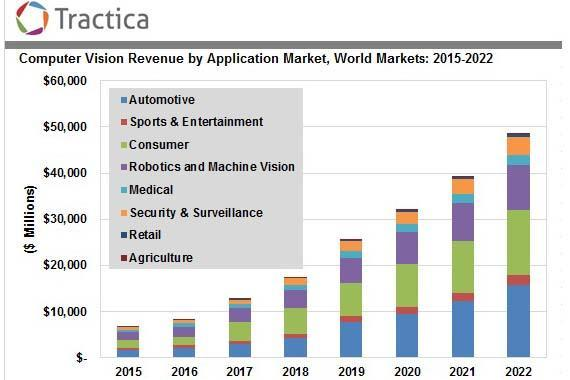
\includegraphics[width=0.8\linewidth]{cv_forecast_2022}
	\caption{Computer Vision revenues in the last years, and forecast for 2022 (source: \cite{cv_forecast}).}
	\label{fig:1_cv_forecast}
\end{figure}


\begin{figure}[h]
	\centering
	\begin{subfigure}[t]{0.45\linewidth}
		\centering
		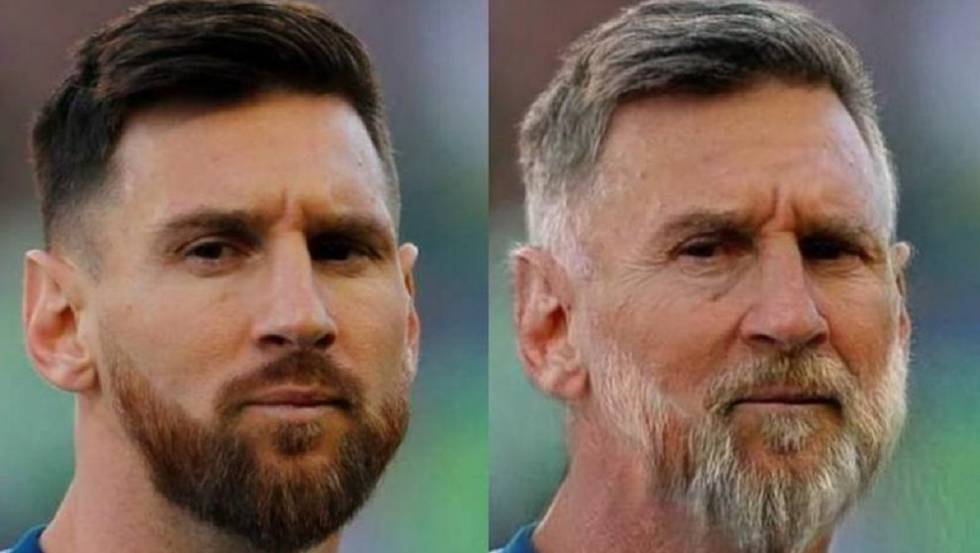
\includegraphics[width=0.8\linewidth]{faceapp_messi}
		\caption{Modifications of a subject on a portrait, such as apparent gender, or age.}
	\end{subfigure}
	\begin{subfigure}[t]{0.45\linewidth}
		\centering
		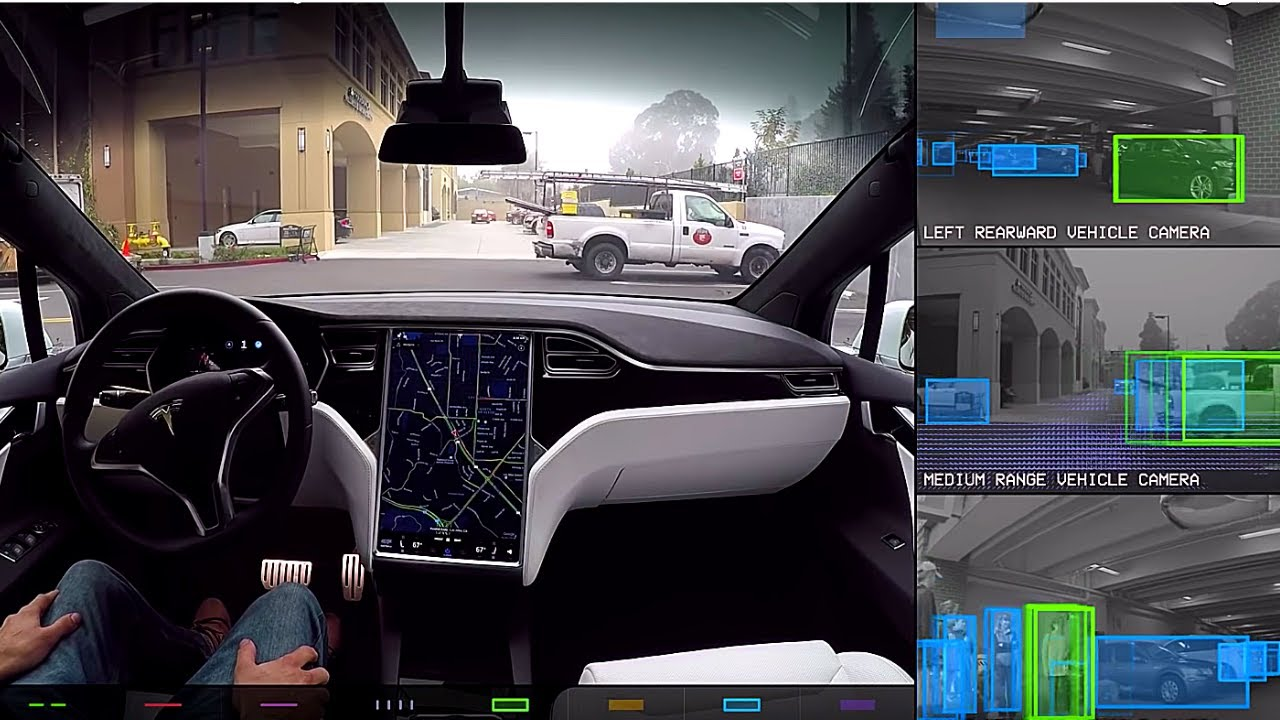
\includegraphics[width=0.95\linewidth]{tesla_autonomous_driving}
		\caption{Autonomous driving on a Tesla Model X.}
	\end{subfigure}
	\caption{Examples of contemporary computer-vision applications.}
	\label{fig:1_computer_vision_applications}
\end{figure}

Specially, the latest times have been notoriously active in this field because of the massive use of \textit{deep learning} for addressing high complexity tasks, such as language understanding \cite{gpt2}, speech recognition \cite{speech_neural} and computer vision problems, which are linked to the growing interest shown in \autoref{fig:1_cv_forecast}. This massive use began in the ImageNet classification contest, where a deep neural network system, AlexNet \cite{alexnet}, achieved an overwhelming victory over other approaches \cite{diapos_deep_learning}. This discovery, along with the significant advances in computing power and parallel computing, has stimulated the usage of these technologies, which show an outstanding performance with the available means nowadays \cite{diapos_deep_learning}.\\


Moreover, robotics applications can be really useful at daily tasks. These tasks are of greater interest when the behavior of a robot tends to emulate the human one, or even pets\footnote{\url{https://www.engadget.com/2018/01/08/new-sony-aibo-first-impressions/}}, with the advantage of no people exposed to a significant risk, or, in a less gloomy scenario, without human body physical limitations. This requires a polished (and somehow complex) behavior, which is triggered by a certain input. At this point, two main branches emerge in robotics:
\begin{description}
	\item [Teleoperated robots:] this kind of robots are capable of performing certain actions, which are \textit{remotely controlled by a human operator}. This type is the mostly used one on hazardousness (\autoref{fig:1_pioneer}) \cite{chernobyl-robot} or high-precision environments \cite{teleop-surgery}. Some advances are made nowadays improving the teleoperation function, implementing \textit{feedback} from the robot, such as haptic feedback \cite{teleop-haptic}, or VR (\emph{Virtual Reality}) sensation, to allow that person to sense the environment as if they were in the robot position.
	
	\item [Autonomous robots:] these robots are much more complex machines, as they are distinguished for implementing a response by themselves, independently of any kind of remote operator. This is seeked on certain scenarios, where there are some factors (as the time elapsed performing an action, or the cost of a control link with the robot) with a considerable weight in the design \cite{ai-space}. This is the kind of robots that concern us on this work: the state-of-the-art techniques try to emulate \textit{human behavior} (\autoref{fig:1_pepper}), so some actions can begin to be performed autonomously with a certain intelligence, as it will be described below.
\end{description}


\begin{figure}[h]
	\centering
	\begin{subfigure}[t]{0.45\textwidth}
		\centering
		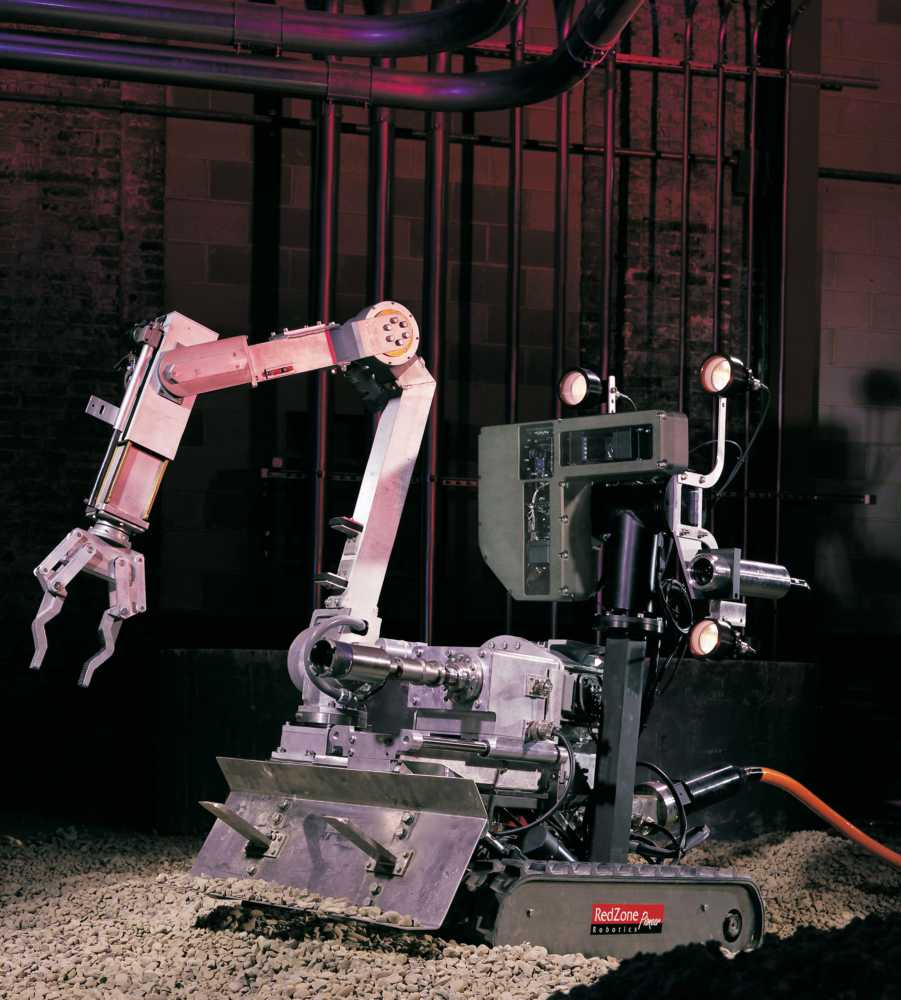
\includegraphics[width=0.8\linewidth]{pioneer_chernobyl}
		\caption{Pioneer robot, designed to perform hazardous teleoperated explorations in a deadly radioactive environment.}
		\label{fig:1_pioneer}
	\end{subfigure}
	\hfill
	\begin{subfigure}[t]{0.4\textwidth}
		\centering
		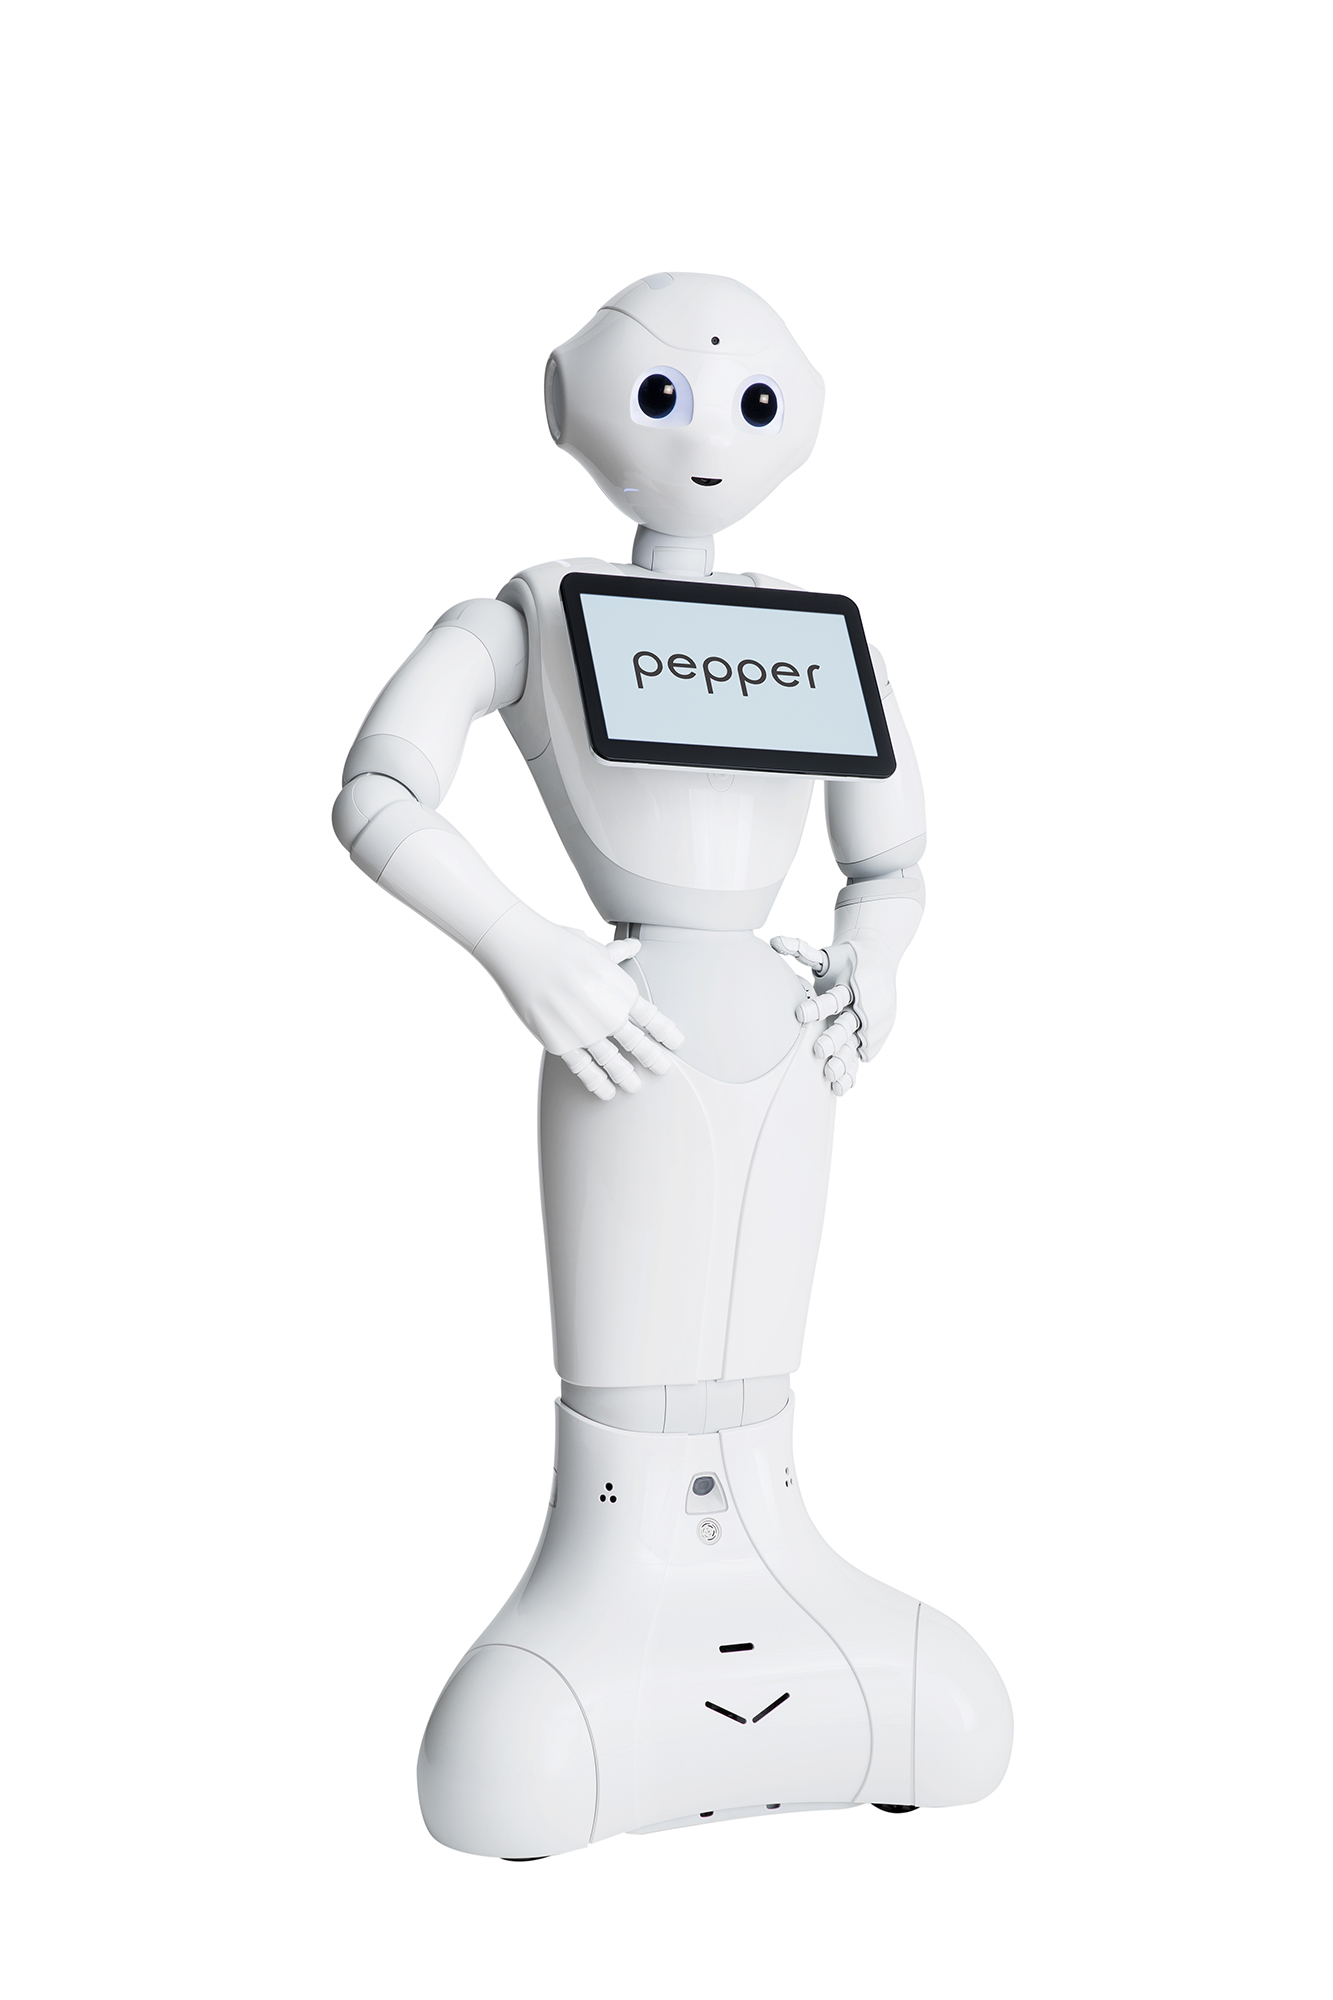
\includegraphics[width=0.8\linewidth]{pepper}
		\caption{Pepper, an autonomous humanoid capable of performing on-board processing and reacting to external stimuli intelligently.}
		\label{fig:1_pepper}
	\end{subfigure}
	\caption{Example of a teleoperated (a) and an autonomous (b) robot.}
	\label{fig:1_robots}
\end{figure}

The important advances on the last decades on the image processing and audio recognition fields have fostered the development of personal assistants, apart from critical machines as the previously described examples.\\



There are outstanding synergies between robotics and computer vision, as it is explored on the system proposed in this work: these fields are combined for obtaining a robust robot capable of following a certain person, navigating towards them on a reactive behavior, and using deep-learning based visual perception. This behavior is composed of two main components: the \textit{perception block}, in charge of processing the images from an embedded RGBD camera, and the \textit{actuation block}, which moves the robotic base accordingly to the relative position of the person to be followed.\\

This application can be specially interesting on social robots, which are designed to follow a person at home or in a hospital. According to \cite{natural_personfollowing}: ``\textit{robots that operate around people in the real world need to move in coherent, easily-understood ways, so that they will not startle or harm the people around them. In particular, for robots that operate in hospitals or in nursing homes}''. 



The work proposed in this thesis improves the system developed on \cite{tfg}, where a neural-network-based following system was run in a standard laptop, with a camera and a robot plugged. In the following dissertation, this work will be revisited, and the points of interest which have allowed to enhance the previous version will be described.\\
	
The main contributions of this dissertation may be summarized as follows:
\begin{description}
	\item[Embedded solution:] the final system is mounted on a battery-powered \textit{mobile base}. This robot features a high-performance GPU embedded on a SoM (\textit{System-on-Module}). In contrast to the previous work, this assembly can operate on its own, without requiring an external computer to perform the deep learning inferences or running algorithms in parallel. A remote monitoring of the behavior is available as well, but it is not required for the system to work. In addition, specific optimization engines allow the system to run faster with 3 neural networks than previously with only 2 networks, on a low-consumption hardware. This will be described in detail in Chapter \ref{chap:4_results}.

	\item[Person identification:] the proposed system runs 3 neural networks. These networks perform inferences over the images captured by the RGBD sensor, which is attached to the system as the sensing source of the robot. The inferences are devoted to detect the different persons in the scene, as well as to distinguish them by means of a discriminant feature: their face. Unlike the previous development, all the detection and identification tasks are based on neural networks, achieving greater robustness and reliability as it will be discussed in Chapter \ref{chap:4_results}.

	\item[Tracking:] the full system includes also a person tracker based on optical flow. This tracker aims to guess the trajectories followed by each person that the robot can see. As opposed to the previous work, this tracker allows to roughly follow the persons while the neural network yields a new update, as this tracker takes considerably less time to predict the person displacement. As a result, the robustness of the entire system is improved, compared to a version governed exclusively by the neural inferences, which are sensitive to visual occlusions as well. Trusting just on these inferences could easily result on an unsteady behavior. However, the introduction of the tracker softens the robot movements ensuring a greater robustness in the observable behavior, as it will be explained on Section \ref{sec:3_design}.
\end{description}


	

\newpage
\section{Objectives}
\label{sec:1_objectives}

	The main objective of this work is to design and develop an embedded system which allows a low-cost robot with a camera to follow a certain person on a robust way. The result will be an autonomous robot which will follow a specific person, whose face has to be known beforehand (using a \textit{reference face} image). This objective, in turn, can be split into specific subgoals:
	
	\begin{enumerate}
		\item Implement a real-time person following behavior using embedded low-power hardware and a low-complexity educational robot.
		
		\item Build the inference pipeline using exclusively CNNs (\textit{convolutional neural networks}), as they offer robustness on detection under harsh lighting conditions, such as the ones observed in \autoref{fig:1_light_ko}.
		
		\begin{figure}[h]
			\centering
			\begin{subfigure}[b]{0.3\linewidth}
				\centering
				
\includegraphics[width=\linewidth]{light_ko}
			\end{subfigure}
%			\hfill
			\begin{subfigure}[b]{0.5\linewidth}
				\centering
				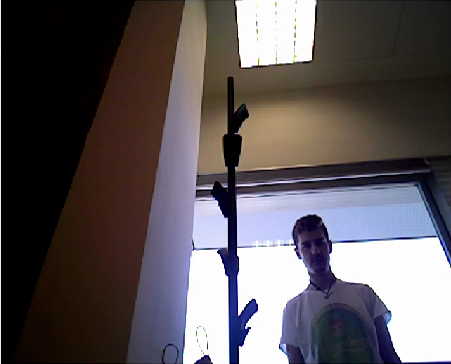
\includegraphics[width=\linewidth]{light_ko_2}
			\end{subfigure}		
			
			\caption{Poor lighting situations for a low-positioned camera.}
			\label{fig:1_light_ko}
		\end{figure}
		
		
		\item Combine a neural visual perception with optical tracking to carry out a robust following of the persons in front of the robot. This will provide the system with extra reliability and robustness against detection losses/occlusions.
	\end{enumerate}
	
These subgoals allow to summarize the starting point for the development of this project: the available materials are an educational robot equipped with a battery, an embedded \textit{SoM} and a RGBD sensor.\\
\newpage
\section{Structure of the document}
\label{sec:1_structure}
The structure of this work is organized as follows:
\begin{itemize}
	\item Chapter \ref{chap:1_introduction} presents the motivation of this work, as well as summarizing the objectives to be addressed.
	\item Chapter \ref{chap:2_sota} discusses the state of the art techniques on person detection and robotic following behaviors, placing the work of this document in a technological frame.
	\item Chapter \ref{chap:3_materials_methods} describes the hardware and software means for developing this work. Later, a full functional description of the implemented system is given, describing the \textit{Perception} and \textit{Actuation} modules that compose the system. Finally, a description of the software architecture that implements the following behavior and makes the robot to follow the person.
	\item Chapter \ref{chap:4_results} describes the experiments conducted on the subsystems and modules of this work. The results of each test are shown as well in order to demonstrate the convenience of the design decisions made over the project development. Finally, a global system experiment is shown, where the following behavior  of the robot has been studied.
	\item Chapter \ref{chap:5_discussions} discusses the obtained results. Later, conclusions are drawn from the developed work, revisiting the goals and subgoals presented above, and proposing future lines of work that can improve the robot and address its main drawbacks.
\end{itemize}

The \hyperref[chap:6_annexes]{Annexes} provide additional tables and results, as it will be mentioned later.


